% SoundCode system architecture block diagram.
% Producer (vLLM AsyncLLMEngine), structural boundary detector,
% async verifier pool (rust-analyzer / cargo check / pyright / etc.),
% checkpoint table, consumer loop. Optional ROCODE LogitsProcessor.
\documentclass[border=2pt]{standalone}
\usepackage{tikz}
\usepackage{xcolor}
\usetikzlibrary{shapes.geometric, arrows.meta, positioning, fit, backgrounds, calc}

\begin{document}
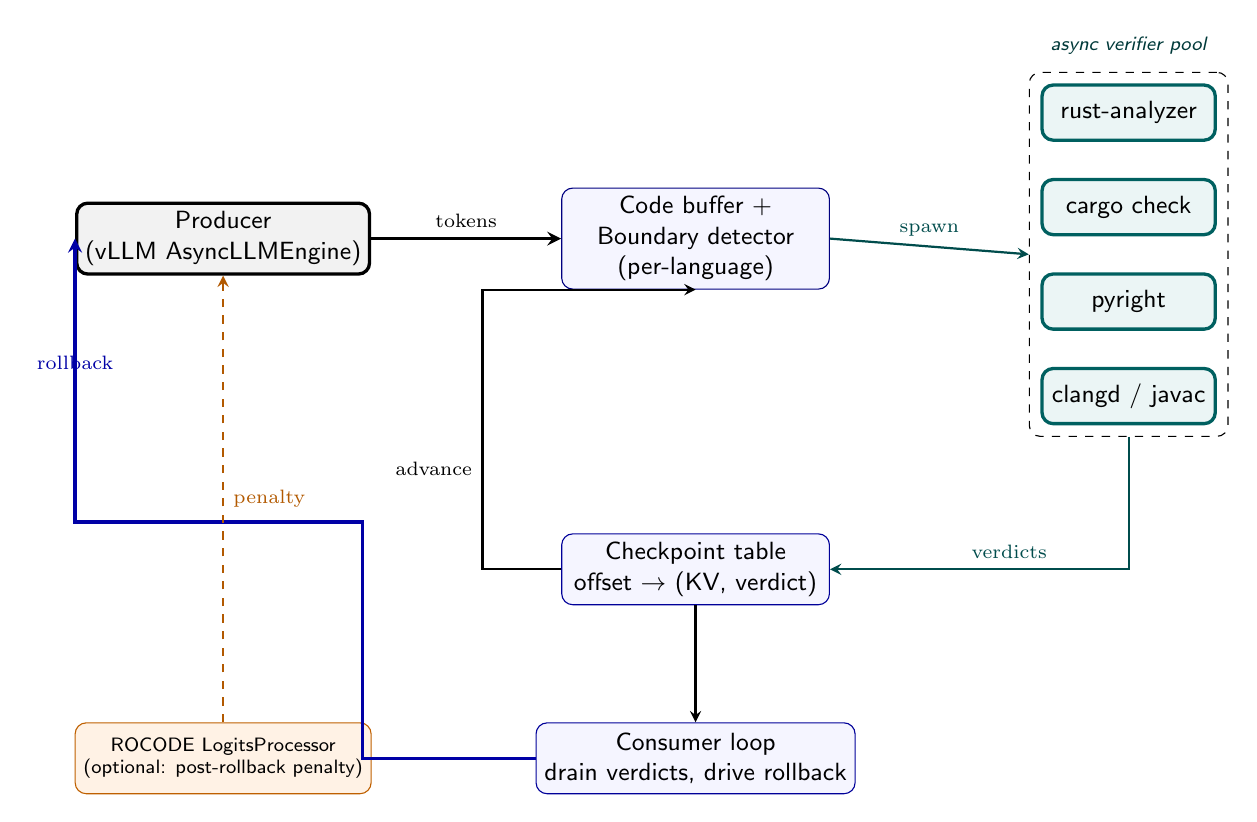
\begin{tikzpicture}[
    >=stealth,
    font=\sffamily\small,
    box/.style       ={draw, rounded corners, align=center, minimum height=9mm,
                       minimum width=30mm, inner sep=3pt, fill=white},
    producer/.style  ={box, fill=black!5, minimum width=36mm, very thick},
    detect/.style    ={box, fill=blue!4, minimum width=34mm,
                       draw=blue!50!black},
    pool/.style      ={box, fill=teal!8, draw=teal!75!black, very thick,
                       minimum width=22mm, minimum height=7mm},
    tablebox/.style  ={box, fill=blue!4, draw=blue!60!black,
                       minimum width=34mm},
    consumer/.style  ={box, fill=blue!4, draw=blue!60!black, minimum width=34mm},
    logits/.style    ={box, fill=orange!10, draw=orange!75!black,
                       minimum width=36mm, font=\sffamily\scriptsize, align=center},
    flow/.style      ={->, thick},
    asyncflow/.style ={->, thick, teal!60!black},
    rollflow/.style  ={->, very thick, blue!65!black},
    penaltyflow/.style={->, thick, orange!70!black, dashed},
    group/.style     ={draw, dashed, rounded corners, inner sep=4pt}
]

% =================== Producer (top-left) ===================
\node[producer] (vllm) at (0,0) {Producer\\(vLLM AsyncLLMEngine)};

% =================== Boundary detector (top-center) ===================
\node[detect] (det) at (6.0,0) {Code buffer +\\Boundary detector\\(per-language)};

% =================== Verifier pool (right column, vertical stack) ===================
\node[pool] (ra) at (11.5,1.6) {rust-analyzer};
\node[pool] (cc) at (11.5,0.4) {cargo check};
\node[pool] (py) at (11.5,-0.8) {pyright};
\node[pool] (cl) at (11.5,-2.0) {clangd / javac};
\node[group, fit=(ra) (cc) (py) (cl),
      label={[font=\sffamily\scriptsize\itshape, text=teal!45!black,
              anchor=south, yshift=1mm]north:async verifier pool}] (poolg) {};

% =================== Checkpoint table (mid-row, below detector) ===================
\node[tablebox] (ckpt) at (6.0,-4.2) {Checkpoint table\\offset $\to$ (KV, verdict)};

% =================== Consumer loop (bottom-center) ===================
\node[consumer] (cons) at (6.0,-6.6) {Consumer loop\\drain verdicts, drive rollback};

% =================== ROCODE LogitsProcessor (bottom-left annotation) ===================
\node[logits] (lp) at (0,-6.6)
    {ROCODE LogitsProcessor\\(optional: post-rollback penalty)};

% --- Arrows ---

% Producer -> detector (top edge: tokens)
\draw[flow, very thick] (vllm.east) -- (det.west)
    node[midway, above, font=\scriptsize] {tokens};

% Detector -> pool (spawn) -- horizontal
\draw[asyncflow] (det.east) -- (poolg.west)
    node[midway, above, font=\scriptsize] {spawn};

% Pool -> ckpt (verdicts) -- around the bottom-right of pool to right of ckpt
\draw[asyncflow] (poolg.south) |- (ckpt.east)
    node[pos=0.7, above, font=\scriptsize] {verdicts};

% ckpt -> consumer (down)
\draw[flow] (ckpt.south) -- (cons.north);

% Advance: ckpt -> detector (left side of both)
\draw[flow] (ckpt.west) -- ++(-10mm,0) |- (det.south)
    node[pos=0.18, left, font=\scriptsize] {advance};

% Consumer -> producer (rollback) -- go down a bit, left around the LogitsProcessor, up to producer west edge
\draw[rollflow] (cons.west) -- ++(-22mm,0) -- ++(0,3.0)
    coordinate (rmid) -- (rmid -| vllm.west) -- (vllm.west)
    node[pos=0.5, above, font=\scriptsize] {rollback};

% Optional LogitsProcessor -> producer (penalty) -- straight up
\draw[penaltyflow] (lp.north) -- (vllm.south -| lp.north)
    node[midway, right, font=\scriptsize] {penalty};

\end{tikzpicture}
\end{document}
